% This is samplepaper.tex, a sample chapter demonstrating the
% LLNCS macro package for Springer Computer Science proceedings;
% Version 2.20 of 2017/10/04
%
\documentclass[runningheads]{llncs}
%
\makeatletter
\usepackage[algoruled,boxed,lined]{algorithm2e}
\makeatletter
\g@addto@macro{\@algocf@init}{\SetKwInOut{Parameter}{Parameters}}
\makeatother
\usepackage{amsmath}
\usepackage{amssymb}
\usepackage{graphicx}

% Used for displaying a sample figure. If possible, figure files should
% be included in EPS format.
%
% If you use the hyperref package, please uncomment the following line
% to display URLs in blue roman font according to Springer's eBook style:
% \renewcommand\UrlFont{\color{blue}\rmfamily}
\usepackage{tikz}
\usetikzlibrary{trees}
\usetikzlibrary{automata, positioning}
\usepackage{listings}
\lstset{basicstyle=\ttfamily}
\usepackage{tcolorbox}
\usepackage{framed}
\usepackage{forest}
\usepackage{xcolor}
\usepackage{blkarray}
\usepackage{comment}
\usepackage{footnote}


\renewcommand{\Coloneqq}{\mathrel{\mathop{::}}=}

\lstdefinestyle{lstStyle}{
	language=C++,
	basicstyle=\small\ttfamily,
	tabsize=4,
	breaklines=true,
	showtabs=false,
	showspaces=false,
	showstringspaces=false,
	columns=flexible
}

\begin{document}
%
	\title{syntaktische Mehrdeutigkeiten beim Parsen}
%
%\titlerunning{Abbreviated paper title}
% If the paper title is too long for the running head, you can set
% an abbreviated paper title here
%
	\author{Lennart Protte\inst{1}}
%
	\authorrunning{Author}
% First names are abbreviated in the running head.
% If there are more than two authors, 'et al.' is used.
%
	\institute{RWTH Aachen University \email{lennart.protte@rwth-aachen.de}}
%
	\maketitle              % typeset the header of the contribution
%
	\begin{abstract}
		Syntaktische Mehrdeutigkeiten stellen eine zentrale Herausforderung beim Parsen von Programmiersprachen dar.
		Diese vorliegende Arbeit untersucht die Auswirkungen solcher Mehrdeutigkeiten
		und betrachtet dabei Ansätze zu ihrer Erkennung, Vermeidung und Auflösung.
		Dabei werden die Vor- und Nachteile von mehrdeutigen Sprachen und Grammatiken diskutiert
		und die Auswirkungen auf das Parsen beleuchtet.
		Um diese Problematik zu lösen,
		wurden Strategien und Algorithmen zur Erkennung und behebung syntaktischer Mehrdeutigkeiten diskutiert.
		Es zeigt sich, dass die Vermeidung von Mehrdeutigkeiten in Grammatiken
		ein einfacheres Parsen ermöglicht, allerdings nicht immer sinnvoll ist.
		Die Arbeit stellt praxistaugliche Methoden zur Erkennung und Auflösung von Mehrdeutigkeiten vor
		und zeigt wie Parser-Techniken dieser Problematik begegnen.

		Die Abwägung zwischen der Einfachheit der Grammatik und der Lesbarkeit der Sprache zeigt,
		dass eindeutige Sprachkonzepte die Komplexität des Parsens reduzieren können,
		aber Mehrdeutigkeiten dennoch nicht immer ein Hindernis darstellen müssen.

		\keywords{Parserbau, syntaktische Mehrdeutigkeiten, Sprachkonzeption}
	\end{abstract}


	\section{Einführung}\label{sec:einfuhrung}
	Bei der Handhabung von Mehrdeutigkeiten, bietet es sich an, die Grammatiken der Sprachen zu betrachten.
	Dabei stellt sich die Frage nach der Definition von Mehrdeutigkeit
	und nach der Bedeutung von Mehrdeutigkeiten für die syntaktische Analyse im Parserbau.

	Die Definition einer mehrdeutigen Grammatik lässt isch wie folgt ausdrücken:
	``Eine Grammatik ist genau dann mehrdeutig, wenn es mindestens eine Eingabe gibt, die mehrere Parse-Bäume besitzt.''
	Daher ist eine Grammatik mehrdeutig, wenn ein Wort der Grammatik über mehrere Wege abgeleitet werden kann.

	Bei Mehrdeutigkeiten lässt sich zwischen lexikalischer und syntaktischer Mehrdeutigkeit unterscheiden.
	Lexikalische Mehrdeutigkeiten treten auf, wenn ein Token mehrere Bedeutungen haben kann.
	Ein Beispiel hierfür ist die lexikalische Mehrdeutigkeit des Tokens ``+'' in der Programmiersprache Java.

	In Java kann das Token ``+'' sowohl als arithmetischer Operator,
	als auch als Konkatenationsoperator von Strings verstanden werden.

	\begin{verbatim}
		//Hier wird der Operator als arithmetischer Operator verwendet
		int a = 1 + 2;
		//Hier wird der Operator als Konkatenationsoperator verwendet
		String b = "Hello" + "World";
	\end{verbatim}

	Solche lexikalischen Mehrdeutigkeiten werden im Lexer behandelt und im Weiteren nicht näher betrachtet.

	Syntaktische Mehrdeutigkeiten hingegen entstehen durch die Struktur der Grammatik selbst.
	Das wohl bekannteste Beispiel dafür ist das ``Dangling else''-Problem,
	welches in vielen bekannten Programmiersprachen auftritt.

	Eine beispielhafter Ausschnitt aus den Produktionsregeln einer Grammatik, die den Syntax eines if-else-Statements beschreibt,
	ist der folgende:


	\begin{align*}
		& P = \{ \begin{aligned}[t]
			         \\
			         ausdruck & \rightarrow \textbf{if} \ bedingung \ \textbf{then} \ ausdruck \\
			         ausdruck & \rightarrow \textbf{if} \ bedingung \ \textbf{then} \ ausdruck \ \textbf{else} \ ausdruck \\
		\end{aligned} \\
		& \}
	\end{align*}

	Wie zu erkennen ist, ist diese Grammatik mehrdeutig, da unklar ist,
	welcher ``else''-Block zu welchem ``if''-Block gehört.
	Im folgenden sind zwei unterschiedliche Interpretationen des Wortes
	``if $\dots$ then if $\dots$ then $\dots$ else $\dots$'' dargestellt.

	\begin{figure}
		\centering
		\begin{forest}
		[\textit{ausdruck}
		[\textbf{if}]
		[\textit{bedingung}]
		[\textbf{then}]
		[\textit{ausdruck}
		[\textbf{if}]
		[\textit{bedingung}]
		[\textbf{then}]
		[\textit{ausdruck}]
		[\textbf{else}]
		[\textit{ausdruck}]
		]
		]
		\end{forest}
		\caption{Hier wird der else-Block der inneren if-Abfrage zugeordnet.}
		\label{fig:figure}
	\end{figure}

	\begin{figure}
		\centering
		\begin{forest}
		[\textit{ausdruck}
		[\textbf{if}]
		[\textit{bedingung}]
		[\textbf{then}]
		[\textit{ausdruck}
		[\textbf{if}]
		[\textit{bedingung}]
		[\textbf{then}]
		[\textit{ausdruck}]
		]
		[\textbf{else}]
		[\textit{ausdruck}]
		]
		\end{forest}
		\caption{In diesem Parse-Baum wird der else-Block der äußeren if-Abfrage zugeordnet.}
		\label{fig:figure2}
	\end{figure}

	Wie hier zu erkennen ist,
	können syntaktische Mehrdeutigkeiten zu unterschiedlichen Interpretationen desselben Quellcodes führen.
	Die Problematik dessen wird im Folgenden behandelt.


	\section{Problemstellung}

	Die Problematik von Mehrdeutigkeiten in Grammatiken besteht darin,
	dass ein Parser keinen eindeutigen Parse-Baum für ein zu parsendes Programm erzeugen kann.
	Wenn Mehrdeutigkeiten bei der Konzeption einer Programmiersprache nicht vermieden werden können,
	muss der Parser in der Lage sein, diese zu parsen.
	Um die korrekte Struktur eines mehrdeutigen Programmes zu ermitteln benötigt ein Parser
	entweder zusätzliche Informationen oder eine bestimmte Vorgehensweise.
	Mehrdeutigkeiten die nicht aufgelöst werden können, da die Sprache inhärent Mehrdeutig ist,
	werden an den Programmierer weitergegeben und erschweren die Entwicklung in der jeweiligen Sprache.



	\begin{figure}
		\centering
		\begin{minipage}{0.48\textwidth}
			\begin{lstlisting}[style=lstStyle,label={lst:lstlisting1}]
class A {public: void func() {}};
class B {public: void func() {}};
class C: public A, public B {};
int main() {
	C c;
	c.func();
	return 0;
}
			\end{lstlisting}
		\end{minipage}
		\hfill
		\begin{minipage}{0.48\textwidth}
			\begin{lstlisting}[style=lstStyle,label={lst:lstlisting2}]
class A {public: void func() {}};
class B {public: void func() {}};
class C: public A, public B {};
int main() {
	C c;
	c.A::func();
	return 0;
}
			\end{lstlisting}
		\end{minipage}
		\caption{Mehrdeutigkeit in der Mehrfachvererbung in C++}
		\label{fig:figure3}
	\end{figure}

	An diesem Beispiel wird deutlich,
	wieso es nicht sinnvoll ist, Mehrdeutigkeiten an den Entwickler weiterzugeben.
	Der Code in Listing \ref{lst:lstlisting1} ist mehrdeutig und wird auch als fehlerhaft erkannt.
	Die Mehrdeutigkeit kommt zu Stande, da die Klasse C von den Klassen A und B erbt,
	die beide eine Methode mit dem Namen ``func'' besitzen.
	Beim Aufruf der Methode ``func'' auf einem Objekt der Klasse C ist unklar,
	ob die Methode von der Oberklasse A oder B aufgerufen werden soll.
	Diese Mehrfachvererbung führt dazu, dass sich nun der Entwickler mit dieser Mehrdeutigkeit auseinandersetzen muss.
	Dies passiert nur, weil die Sprache C++ keine explizite Angabe der Klasse bei einem Methodenaufruf verlangt.

	Wenn Mehrdeutigkeiten nicht vermieden werden können,
	kann der Ansatz versucht werden, diese zu erkennen und aufzulösen.
	Dies kann jedoch die Laufzeit eines Parsers beeinträchtigen und sollte daher gut abgewogen werden.
	Während eindeutige Sprachen einfach und effizient, beispielsweise mit einem LR-Parser, geparst werden können,
	ist das Parsen von mehrdeutigen Sprachen komplexer und weniger effizient.

	Eine weitere Problematik ist, dass es theoretisch nicht möglich ist zu entscheiden,
	ob eine gegebene Grammatik mehrdeutig ist oder nicht.
	Dieses Problem, auch bekannt als Post'sche Korrespondenzproblem
	spielt vor allem in der Konzeption neuer Programmiersprachen eine Rolle.
	Dieses Problem wird im nächsten Abschnitt genauer erläutert.


	\section{Vermeidung von Mehrdeutigkeiten}\label{sec:vermeidung-von-mehrdeutigkeiten}

	Da Mehrdeutigkeiten in Grammatiken sowohl in der Entwicklung des Parsers,
	als auch in der Anwendung der Sprache hinderlich sein können,
	ist es sinnvoll Mehrdeutigkeiten von vornherein zu vermeiden.
	Um eine Sprache eindeutig zu gestalten,
	muss die Grammatik der Sprache so konzipiert werden,
	dass es für jedes Wort der Sprache nur einen Parse-Baum gibt.
	So können wir Beispielsweise die obige Grammatik des ``Dangling else''-Problems auch wie folgt realisieren\cite{Abrahams1966}:

	\begin{align*}
		& P = \{ \begin{aligned}[t]
			         \\
			         ausdruck & \rightarrow ausdruck_{auf} | ausdruck_{zu} \\
			         ausdruck_{auf} & \rightarrow \textbf{if} \ bedingung \ \textbf{then} \ ausdruck \\
			         \phantom{A} & \phantom{\rightarrow} \vert \textbf{if} \ bedingung \ \textbf{then} \ ausdruck_{zu} \ \textbf{else} \ offener\_ausdruck \\
			         ausdruck_{zu} & \rightarrow \textbf{if} \ bedingung \ \textbf{then} \ ausdruck_{zu} \ \textbf{else} \ ausdruck_{zu} \\
		\end{aligned} \\
		& \}
	\end{align*}

	Dadurch, dass nun zwischen offenen und geschlossenen ``if''-Blöcken unterschieden wird,
	kann diese Grammatik eindeutig von einem LR-Parser verarbeitet werden.

	Das Festlegen von zusätzlichen Regeln wie Vorrangsregeln und Assoziativität,
	macht die Grammatik nicht direkt eindeutig,
	ermöglicht es aber diese in eine eindeutige Form zu bringen.

	Allerdings kann es auch Nachteile haben, eine Sprache eindeutig zu gestalten.
	So ist die Grammatik einer mehrdeutigen Sprache oft einfacher, kürzer und intuitiver als die einer eindeutigen Sprache.
	Auch können die Eindeutigkeitsanforderungen an eine Sprache schnell Boilerplate-Code verursachen.

	\begin{figure}
		\begin{lstlisting}[style=lstStyle,label={lst:lstlisting3}]
			public class Main {
			    public static void main(String[] args) {
			        System.out.println("Hello, World!");
			    }
			}
		\end{lstlisting}
		\caption{Beispiel für Boilerplate-Code in Java}
		\label{fig:figure4}
	\end{figure}

	Dieses Beispiel der Sprache Java zeigt, dass zu große Eindeutigkeitsanforderungen,
	hier in Form von Sichtbarkeitsmodifikatoren und Typenangaben, schnell zu verbosem Code führen können.
	Es ist daher eine Abwägung zwischen der Einfachheit des Parsers und der Komplexität und Lesbarkeit der Sprache zu treffen.


	\section{Erkennung von Mehrdeutigkeiten}\label{sec:erkennung-von-mehrdeutigkeiten}

	Um eine eindeutige Grammatik für eine Sprache zu entwerfen,
	ist es notwendig diese Grammatik auf Mehrdeutigkeiten zu überprüfen.
	Dazu eignen sich Suchalgorithmen, die durch die Ableitungen der Grammatik traversieren
	und dabei auf Mehrdeutigkeiten prüfen.
	Dabei ist zu beachten, dass die Überprüfung, ob eine Grammatik mehrdeutig ist oder nicht,
	unentscheidbar ist.\cite{hopcroft2006introduction}
	Statistisch gesehen ist es wahrscheinlicher eine Mehrdeutigkeiten bei einer Breitensuche zu finden,
	als bei einer Tiefensuche.\cite{springer2013}
	Der ``dynamic1''-Algorithmus\cite{springer2013} ist ein nicht-deterministischer Algorithmus,
	welcher zufällige Ableitungsalternativen wählt und dabei bis zu einer festgelegten Tiefe traversiert.
	Wenn der Algorithmus diese Tiefe erreicht hat, bevorzugt er Alternativen, welche zuvor noch gar nicht oder
	verhältnismäßig selten gewählt oder weniger bis keine nicht-Terminalsymbole enthalten.
	Allerdings kann es auch bei diesem Algorithmus dazu kommen, dass er nicht terminiert.
	In einem Experiment\cite{springer2013} zeigte sich,
	dass der ``dynamic1''-Algorithmus eine Verbesserung zu ACLA, AMBER und AmbiDexter darstellt.
	Zwar übersieht er teilweise Mehrdeutigkeiten, die von den anderen Algorithmen gefunden wurden,
	aber insgesamt findet er zum einen mehr und zum anderen deutlich tiefer verschachtelte Mehrdeutigkeiten.


	\section{Auflösung von Mehrdeutigkeiten}\label{sec:auflosung-von-mehrdeutigkeiten}

	Sollte eine Grammatik mehrdeutig sein, so muss ein Parser in der Lage sein, diese Mehrdeutigkeiten aufzulösen.
	Konkret bedeutet dies, dass zusätzliche Regeln
	wie beispielsweise Assoziativität und Vorrangregeln für Operatoren festgelegt werden müssen,
	unter welchen die Grammatik in eine eindeutige Form gebracht werden kann.
	Dazu eignet sich ein Algorithmus\footnotemark[1], welcher die gebenen Regeln auf die Grammatik anwendet
	und sie so in eine eindeutige Form transformiert.
	Der Algorithmus arbeitet mit so gennanten ``Mustern zur Beseitigung von Mehrdeutigkeiten''.
	Ein Muster ist ein vier-Tupel $(S, \alpha \circ \beta, \gamma)$, mit $S$ als das Startsymbol der Produktion,
	$\alpha \circ \beta$ sind zwei Nichtterminale aus $G$ mit $\circ$ als Operator und $\gamma$ ist die gewählte Ableitung, wobei
	$\bullet$ markiert, ob $\alpha$ oder $\beta$ abgeleitet wird.
	Mithilfe von diesen Mustern können Tabellen\footnotemark[2] für unsere zwei binären Operatoren $+$ und $*$ aufgestellt werden:

	\begin{figure}
		\centering
		\begin{tabular}{|c|c|}
			\hline
			& $E \Coloneqq E\alpha_{2}E$                   \\
			\hline
			$E \Coloneqq E\alpha_{1}E$ & $(E, \bullet{E}\alpha_{1}E, {E}\alpha_{2}E)$ \\
			& $(E, E\alpha_{1}\bullet{E}, E\alpha_{2}E)$   \\
			\hline
		\end{tabular}
		\caption{Tabelle für Vorrangsregeln}
		\label{fig:figure5}
	\end{figure}

	Diese Tabelle zeigt, dass der Operator $\alpha_{1}$ Vorrang vor dem Operator $\alpha_{2}$ hat,
	daher immer zuerst abgeleitet wird.

	\begin{figure}
		\centering
		\begin{tabular}{|c|c|c|}
			\hline
			& $E \Coloneqq E\alpha_{1}E$                 & $E \Coloneqq E\alpha_{2}E$                 \\
			\hline
			$E \Coloneqq E\alpha_{1}E$ & $(E, E\alpha_{1}\bullet{E}, E\alpha_{1}E)$ & $(E, E\alpha_{1}\bullet{E}, E\alpha_{2}E)$ \\
			\hline
			$E \Coloneqq E\alpha_{2}E$ & $(E, E\alpha_{2}\bullet{E}, E\alpha_{1}E)$ & $(E, E\alpha_{2}\bullet{E}, E\alpha_{2}E)$ \\
			\hline
		\end{tabular}
		\caption{Tabelle die links-Assotiativität}
		\label{fig:figure6}
	\end{figure}

	Hier ist die Assotiativität festgelegt.
	Wie zu erkennen ist, wird in jeder möglichen Kombination beider Operatoren immer erst das linke Nichtterminal abgeleitet.
	Im Weiteren betrachten wir einen beispielhaften Durchlauf des Algorithmus anhand einer gegebenen Grammatik.
	Angenommen wir haben folgende Grammatik für einfache arithmetische Ausdrücke mit dazu gegebener Assoziativität und Vorrang:

	\begin{figure}
		\begin{minipage}{0.48\textwidth}
			\begin{flushleft}
				\begin{align*}
					& G(N,T,P,S) \\
					& N = \{E\} \\
					& T = \{+, *, \bold{zahl}\} \\
					& S = \{E\} \\
					& P = \{ \begin{aligned}[t]
						         \\ E & \rightarrow E + E | E * E | \bold{zahl}
					\end{aligned} \\
					& \}
				\end{align*}
			\end{flushleft}
		\end{minipage}
		\hfill
		\begin{minipage}{0.48\textwidth}
			\begin{tabular}{|c|c|c|}
				\hline
				Operator & Assoziativität & Priorität \\
				\hline
				+            & links          & 1         \\
				*            & links          & 2         \\
				\hline
			\end{tabular}
		\end{minipage}
		\caption{mehrdeutige Grammatik mit Operator-Assoziativitäten und Vorangregeln}
		\label{fig:figure7}
	\end{figure}

	Der Algorithmus ermittelt nun die Muster zur Beseitigung von Mehrdeutigkeiten und kommt dabei zu folgendem Ergebnis:

	\begin{figure}
		\begin{minipage}{0.48\textwidth}
			\begin{flushleft}
				\begin{align*}
				(E, E*\bullet{E}, E*E)
					\\
					(E, \bullet{E}*E, E+E) \\
					(E, E+\bullet{E}, E*E) \\
					(E, \bullet{E}+E, E+E)
				\end{align*}
			\end{flushleft}
		\end{minipage}
		\hfill
		\begin{minipage}{0.48\textwidth}
			\begin{align*}
				& G(N,T,P,S) \\
				& N = \{E, E_1, E_2, E_3, E_4\} \\
				& T = \{+, *, \bold{zahl}\} \\
				& S = \{E\} \\
				& P = \{ \begin{aligned}[t]
					         \\
					         E &\rightarrow E_1 * E_2 | E_3 + E_4 | \bold{zahl} \\
				\end{aligned} \\
				& \}
			\end{align*}
		\end{minipage}
		\caption{Anwenden der Muster auf die gegebene Grammatik}
		\label{fig:figure8}
	\end{figure}

	Wie hier zu erkennen ist, wurde im ersten Schritt für jedes der Muster ein neues Nichtterminal hinzugefügt.
	Der Algorithmus kopiert die Produktion der Grammatik nun für jedes neu eingeführte Nichtterminal
	und wendet dabei jeweils eines Muster auf die Produktion an.
	In einem weiteren Schritt wird der Prozess dann für verschachtelte Fälle wiederholt.

	\begin{figure}
		\begin{minipage}{0.48\textwidth}
			\begin{flushleft}
				\begin{align*}
					& G(N,T,P,S) \\
					& N= \{E, E_1, E_2, E_3, E_4\} \\
					& T= \{+, *, \bold{num}\} \\
					& S= \{E\} \\
					& P = \{ \\
					& E     \rightarrow E_1 * E_2 | E_3 + E_4 | \bold{num} \\
					& E_1   \rightarrow E_1 * E_2 | \bold{num} \\
					& E_2   \rightarrow E_3 + E_4 | \bold{num} \\
					& E_3   \rightarrow E_1 * E_2 | \bold{num} \\
					& E_4   \rightarrow E_3 + E_4 | \bold{num} \\
					& \}
				\end{align*}
			\end{flushleft}
		\end{minipage}
		\hfill
		\begin{minipage}{0.48\textwidth}
			\begin{align*}
				& G(N,T,P,S) \\
				& N= \{E, E_1, E_2, E_3, E_4, E_5\} \\
				& T= \{+, *, \bold{num}\} \\
				& S= \{E\} \\
				& P = \{ \\
				& E     \rightarrow E_1 * E_2 | E_3 + E_4 | \bold{num} \\
				& E_1   \rightarrow E_1 * E_5 | \bold{num} \\
				& E_2   \rightarrow E_3 + E_4 | \bold{num} \\
				& E_3   \rightarrow E_5 * E_2 | \bold{num} \\
				& E_4   \rightarrow E_3 + E_4 | \bold{num} \\
				& E_5   \rightarrow \bold{num} \\
				& \}
			\end{align*}
		\end{minipage}
		\caption{Erstellung neuer Produktionen und prüfen von Verschachtelungen}
		\label{fig:figure9}
	\end{figure}

	Hier wurde der verschachtelte Fall aufgelöst,
	wo die Multiplikation über einen Zwischenschritt von rechts aufgebaut werden konnte.

	Eine solche Grammatik kann dann effizient und in linearer Zeit von einem LR-Parser verarbeitet werden.
	Ein LR-Parser ist ein Bottom-Up-Parser, der die Produktionen der Grammatik von links nach rechts verarbeitet.
	Er arbeitet mit Shift- und Reduce-Operationen und kann unter Verwendung eines Stack und einer Zustandsmaschine
	die Produktionen der Grammatik in linearer Zeit verarbeiten.

	Eine weitere Möglichkeit Mehrdeutigkeiten in einer gegebenen Grammatik aufzulösen
	ist die Umformung der Grammatik in die Chomsky-Normalform (kurz CNF).
	Bei der Umformung in die CNF können Mehrdeutigkeiten aufgelöst werden, müssen aber nicht.
	Nach der Umformung kann daher keine Aussage über die Mehrdeutigkeit der Grammatik getroffen werden.
	Dennoch kann eine Umformung in die CNF sinnvoll sein, besonders da die Parse-Bäume,
	die aus einer Grammatik in der CNF resultieren, immer Binärbäume sind.

	\footnotetext[1]{Vasudevan, N., Tratt, L. (2013). Detecting Ambiguity in Programming Language Grammars. Seite 149 - 150}
	\footnotetext[2]{Vasudevan, N., Tratt, L. (2013). Detecting Ambiguity in Programming Language Grammars. Seite 147}


	\section{Parsen von Mehrdeutigkeiten}\label{sec:parsen-von-mehrdeutigkeiten}

	Zum Parsen von Mehrdeutigkeiten benötigt es komplexere Parser-Techniken als die klassischen LL- und LR-Parser.
	Um die richtige aus den möglichen Ableitungen zu wählen,
	muss ein Parser in der Lage sein, alle möglichen Ableitungen zu finden.
	Eine Möglichkeit Mehrdeutigkeiten zu parsen sind Lookahead-Parser.
	Lookaheads sind eine Technik, bei der der Parser nicht nur das aktuelle Token betrachtet,
	wie es bei einem LL- oder LR-Parser der Fall ist, sondern auch nachfolgende Tokens.
	Beispielsweise verwendet der ANTLR-Parser-Generator Lookaheads,
	für beliebig viele nachfolgende Tokens.

	Eine weitere Möglichkeit Mehrdeutigkeiten zu parsen sind Chart-Parser.
	Eine Variante davon ist der CYK-Parser,
	dieser benötigt eine Grammatik in der Chomsky-Normalform.

	Wir betrachten beispielhaft unsere mehrdeutige ``Dangline-Else''-Grammatik in der CNF.
	Für das Wort ``\textbf{if} $bedingung$ \textbf{then} \textbf{if} $bedingung$ \textbf{then} $ausdruck$ \textbf{else} $ausdruck$'',
	erstellt der CYK-Parser folgende Tabelle auf:

	\begin{figure}
		\begin{minipage}{0.48\textwidth}
			\begin{flushleft}
				\begin{align*}
					& P = \{ \begin{aligned}[t]
						         \\
						         S & \rightarrow ausdruck \vert CA \vert DA \\
						         A & \rightarrow ausdruck \vert CA \vert DA \\
						         B & \rightarrow bedingung \\
						         C & \rightarrow FE \\
						         D & \rightarrow HG \\
						         E & \rightarrow \bold{then} \\
						         F & \rightarrow IB \\
						         G & \rightarrow \bold{else} \\
						         H & \rightarrow CA \\
						         I & \rightarrow \bold{if} \\
					\end{aligned} \\
					& \}
				\end{align*}
			\end{flushleft}
		\end{minipage}
		\hfill
		\begin{minipage}{0.48\textwidth}
			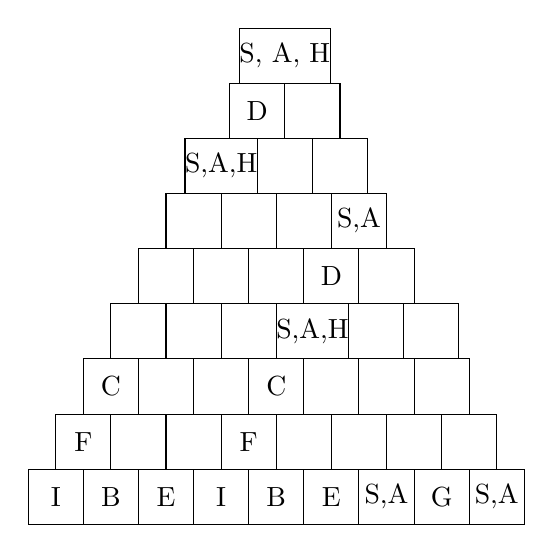
\begin{tikzpicture}[
				node distance = 0pt,
				every node/.style = {draw, minimum size=7mm, inner sep=0pt, outer sep=0pt}
			]
				\node (n1)  {S, A, H};
				%
				\node (n11) [below left=of n1.south]    {D};
				\node (n12) [right=of n11]              {};
				%
				\node (n21) [below left=of n11.south]   {S,A,H};
				\node (n22) [right=of n21]              {};
				\node (n23) [right=of n22]              {};
				%
				\node (n31) [below left=of n21.south]   {};
				\node (n32) [right=of n31]              {};
				\node (n33) [right=of n32]              {};
				\node (n34) [right=of n33]              {S,A};
				%
				\node (n41) [below left=of n31.south]   {};
				\node (n42) [right=of n41]              {};
				\node (n43) [right=of n42]              {};
				\node (n44) [right=of n43]              {D};
				\node (n45) [right=of n44]              {};

				%
				\node (n51) [below left=of n41.south]   {};
				\node (n52) [right=of n51]              {};
				\node (n53) [right=of n52]              {};
				\node (n54) [right=of n53]              {S,A,H};
				\node (n55) [right=of n54]              {};
				\node (n56) [right=of n55]              {};
				%
				\node (n61) [below left=of n51.south]   {C};
				\node (n62) [right=of n61]              {};
				\node (n63) [right=of n62]              {};
				\node (n64) [right=of n63]              {C};
				\node (n65) [right=of n64]              {};
				\node (n66) [right=of n65]              {};
				\node (n67) [right=of n66]              {};
				%
				\node (n71) [below left=of n61.south]   {F};
				\node (n72) [right=of n71]              {};
				\node (n73) [right=of n72]              {};
				\node (n74) [right=of n73]              {F};
				\node (n75) [right=of n74]              {};
				\node (n76) [right=of n75]              {};
				\node (n77) [right=of n76]              {};
				\node (n78) [right=of n77]              {};
				%
				\node (n81) [below left=of n71.south]   {I};
				\node (n82) [right=of n81]              {B};
				\node (n83) [right=of n82]              {E};
				\node (n84) [right=of n83]              {I};
				\node (n85) [right=of n84]              {B};
				\node (n86) [right=of n85]              {E};
				\node (n87) [right=of n86]              {S,A};
				\node (n88) [right=of n87]              {G};
				\node (n89) [right=of n88]              {S,A};

			\end{tikzpicture}
		\end{minipage}
		\caption{CYK-Parser für mehrdeutige Grammatik}
		\label{fig:figure10}
	\end{figure}

	Eine wichtige Anmerkung zu der hier gezeigten Grammatik ist, dass zur besseren Darstellung der Tabelle,
	die Nichtterminale $ausdruck$ und $bedingung$ hier als Terminalsymbole in der Grammatik aufgeführt sind.

	Wie an diesem Ergebnis zu erkennen ist, findet der CYK-Parser hier alle mögliche Ableitungen für das gegebene Wort.
	Mit zusätzlichen Regeln, welcher dieser ableitungen verwendet werden sollen,
	kann somit auch eine mehrdeutige Grammatik geparst werden.

	\section{Fazit}\label{sec:zusammenfassung}

	Abschließend lässt sich festhalten, dass Mehrdeutigkeiten in Grammatiken von Programmiersprachen
	eine zentrale Herausforderung beim Parsen darstellen.
	Durch die Vermeidung und Auflösung von Mehrdeutigkeiten können einfachere Parser verwendet werden.
	Wenn vermieden werden kann, dass Mehrdeutigkeiten an den Entwickler weitergegeben werden,
	erleichtert dies die Entwicklung in der jeweiligen Sprache.
	Dies kann aber auch zu Einschränkungen in der Sprache führen und die Lesbarkeit des Codes beeinträchtigen.
	Mehrdeutige Sprachen sind oft einfacher und intuitiver zu verstehen.
	Die Tatsache, dass viele gängige Programmiersprachen wie C, Java oder Python mehrdeutig sind,
	zeigt, dass Mehrdeutigkeiten in Programmiersprachen praxistauglich sind.
	Neuere Programmiersprachen wie Swift oder C\# hingegen vermeiden oft Mehrdeutigkeiten
	und können daher effizienter, beispielsweise mit einfachen Lookahead-Parsern, geparst werden.
	Dem gegenüber stehen Ansätze wie AppleScript,
	welches einen Syntax ähnlich der natürlichen Sprache besitzt
	und damit besonders einsteigerfreundlich aber eben auch mehrdeutig ist.

	Abschließend sollte festgehalten werden, dass bei der Konzeption einer neuen Programmiersprache
	darauf geachtet werden sollte, keine Mehrdeutigkeiten an den Entwickler weiterzugeben.

%
% ---- Bibliography ----
%
% BibTeX users should specify bibliography style 'splncs04'.
% References will then be sorted and formatted in the correct style.
%


	\nocite{*}
	\bibliographystyle{splncs04}
	\bibliography{refs}
\end{document}
